\chapter{Measurements of the Higgs Boson through Vector Boson Scattering}
\begin{aquote}{Peter Higgs, Edinburgh University press conference, 2012}
    It's very nice to be right sometimes.
\end{aquote}
\section{Introduction}
The stage is set: over a century of particle physics has yielded a beautiful, but incomplete theory of everything, the Standard Model, and a grand coalition of nations have built the largest and most complex scientific instrument in human history, the LHC, to test it. 
The most recent triumph came in 2012, when the Higgs boson was discovered. 
In the years following its discovery, however, the LHC experiments have measured many of its properties to great precision and found no significant deviations from SM predictions~\cite{NatureHiggsCMS2022, NatureHiggsATLAS2022}. 
Nevertheless, the confounding mysteries still surrounding the Higgs boson at the time of writing suggest that there must be some physics beyond the Standard Model (BSM). 
Moreover, given the existential importance of the Higgs boson, this kind of new physics would have profound implications towards a better understanding of the past, present, and future of the entire universe. 

There are many educated guesses, called theories, aimed at addressing these open questions around the Higgs boson. 
To determine their viability, experimentalists can search for the additions directly if, for example, entirely new particles are proposed. 
% And so began the opening pages of several thousand PhD theses, with this being only the latest addition. 
% Detailed amidst their pages are facts and figures, like those presented in this chapter, derived from the statistical analysis of proton-proton collision data collected by the LHC experiments. 
% There are many educated guesses at the answers to those open questions around the Higgs. 
% Physicists at the LHC are in the business of measuring cross sections: how often does a given physical process occur? 
% Then, if that physical process is affected by some new physics, one can compare the measured rate of occurance to that predicted by the new theory. 

\section{Determination of \lambdaWZ through VBS WH}
\subsection{Looking for a sign}
One commonly used framework used to quantify the deviations from the SM is the so-called $k$-framework~\cite{KFrame}, which introduces modifiers $\kappa_X$ to the Higgs boson couplings to some particle $X$:
\begin{equation}
    \kappa_X = \frac{\text{modifed coupling value}}{\text{SM coupling value}}.
\end{equation}
While there are myriad theoretical nuances to the statement above, it is sufficient to state the obvious: $\kappa_X = 1$ represents the SM scenario and significant deviations from 1 represent BSM scenarios. 
Within this framework, the CMS Collaboration had constrained the \textit{magnitudes} of the HWW (\kW) and HZZ (\kZ) couplings to $|\kW| = 1.02^{+0.11}_{-0.10}$ and $|\kZ| = 1.04^{+0.07}_{-0.07}$, showing precise agreement with the SM values~\cite{NatureHiggsCMS2022}. 
The \textit{sign} of either coupling, however, had not yet been well-determined. 

The relative sign between \kW and \kZ can be expressed more compactly as their ratio:
\begin{equation}
    \lambdaWZ = \frac{\kW}{\kZ}.
\end{equation}
The Standard Model requires $\lambdaWZ = 1$ in order to preserve the ``custodial'' symmetry. 
Meanwhile, certain BSM theories, such as so-called ``Higgs doublet'' models, require $\lambdaWZ < 0$. 
Therefore, in the absence of a significant experimental measurement of the sign of \lambdaWZ, a crucial element of the SM had not been confirmed, and a potential indication of BSM had not been explored. 

\subsection{The signal}
The precise determinations of the magnitude of \kW and \kZ~\cite{NatureHiggsCMS2022} were performed by studying processes that are predominantly quadratic in \kW or \kZ---that is, \kW or \kZ enter the Feynman diagram twice. % add a feynman diagram?
While there were some with a linear dependence, they did not give a strong exclusion of opposite-sign scenarios~\cite{BestCMSLambdaWZ}. 
A promising channel to directly probe \lambdaWZ at the LHC is the production of \VH via vector-boson scattering (VBS)~\cite{Theory2LambdaWZ}.
Such a channel is sensitive to the relative sign of \kW and \kZ since the since the cross section $\sigma$ has an interference term that is linear in both \kW and \kZ~\cite{Theory2LambdaWZ}: 
\begin{equation}\label{eq:matrix_elem}
    \sigma \propto |\mathcal{M}|^2 = \kW^2|\mathcal{M}_W|^2 + \kW\kZ\mathcal{M}_{WZ}^2 + \kZ^2|\mathcal{M}_Z|^2
\end{equation}
where the matrix elements for the contributions from the $\PH\PW\PW$ couplings, $\PH\PZ\PZ$ couplings, and interference term are denoted as $\mathcal{M}_W$, $\mathcal{M}_W$, and $\mathcal{M}_{WZ}$ respectively. 
Therefore, this channel provides the possibility to determine with certainty that \lambdaWZ is indeed positive, as the SM predicts.
\begin{figure}[htb]
    \centering
    \subfloat{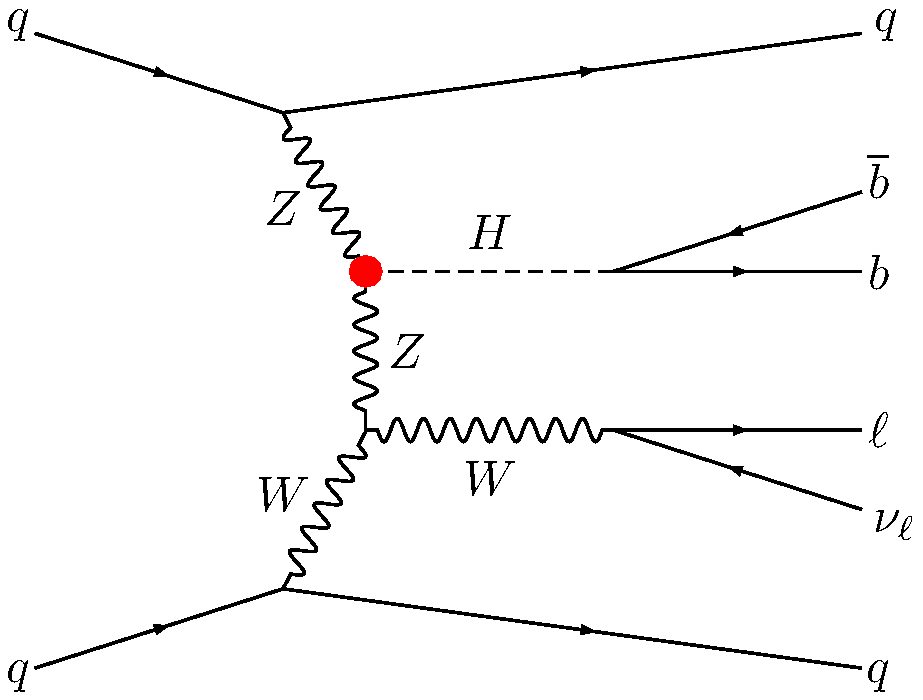
\includegraphics[width=0.3\textwidth]{fig/feynman/vbswh/vbswh_1.pdf}}\quad
    \subfloat{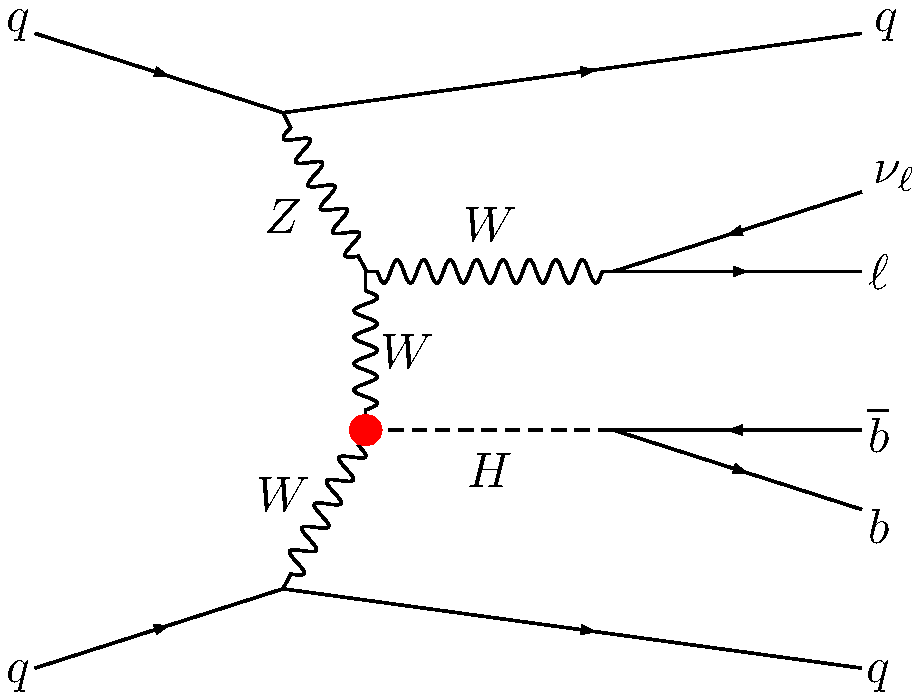
\includegraphics[width=0.3\textwidth]{fig/feynman/vbswh/vbswh_2.pdf}}\quad
    \subfloat{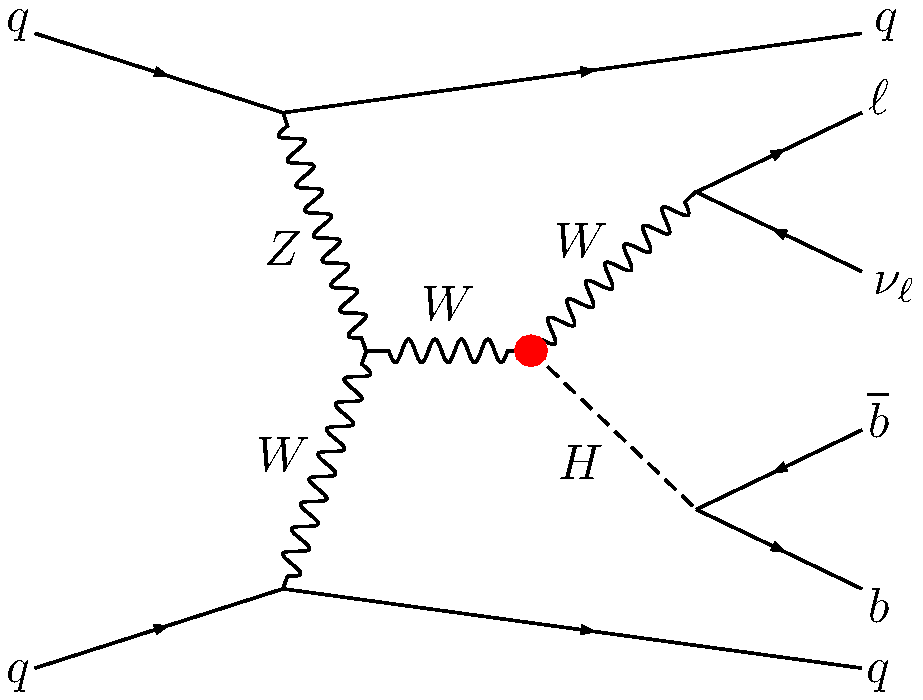
\includegraphics[width=0.3\textwidth]{fig/feynman/vbswh/vbswh_3.pdf}}
    \caption{
        Leading-order Feynman diagrams for VBS production of a W and Higgs boson, where the W decays leptonically and the Higgs decays to b quarks. 
        The Higgs coupling to W bosons \kW and Z bosons \kZ is denoted by a red circle (\textcolor{red}{\ding{108}}). 
    }
    \label{fig:vbswh_feynman}
\end{figure}

\subsection{The backgrounds}
\subsection{Event selection}
\subsection{Background estimation}
\subsection{Results}
\begin{figure}[htb]
    \centering
    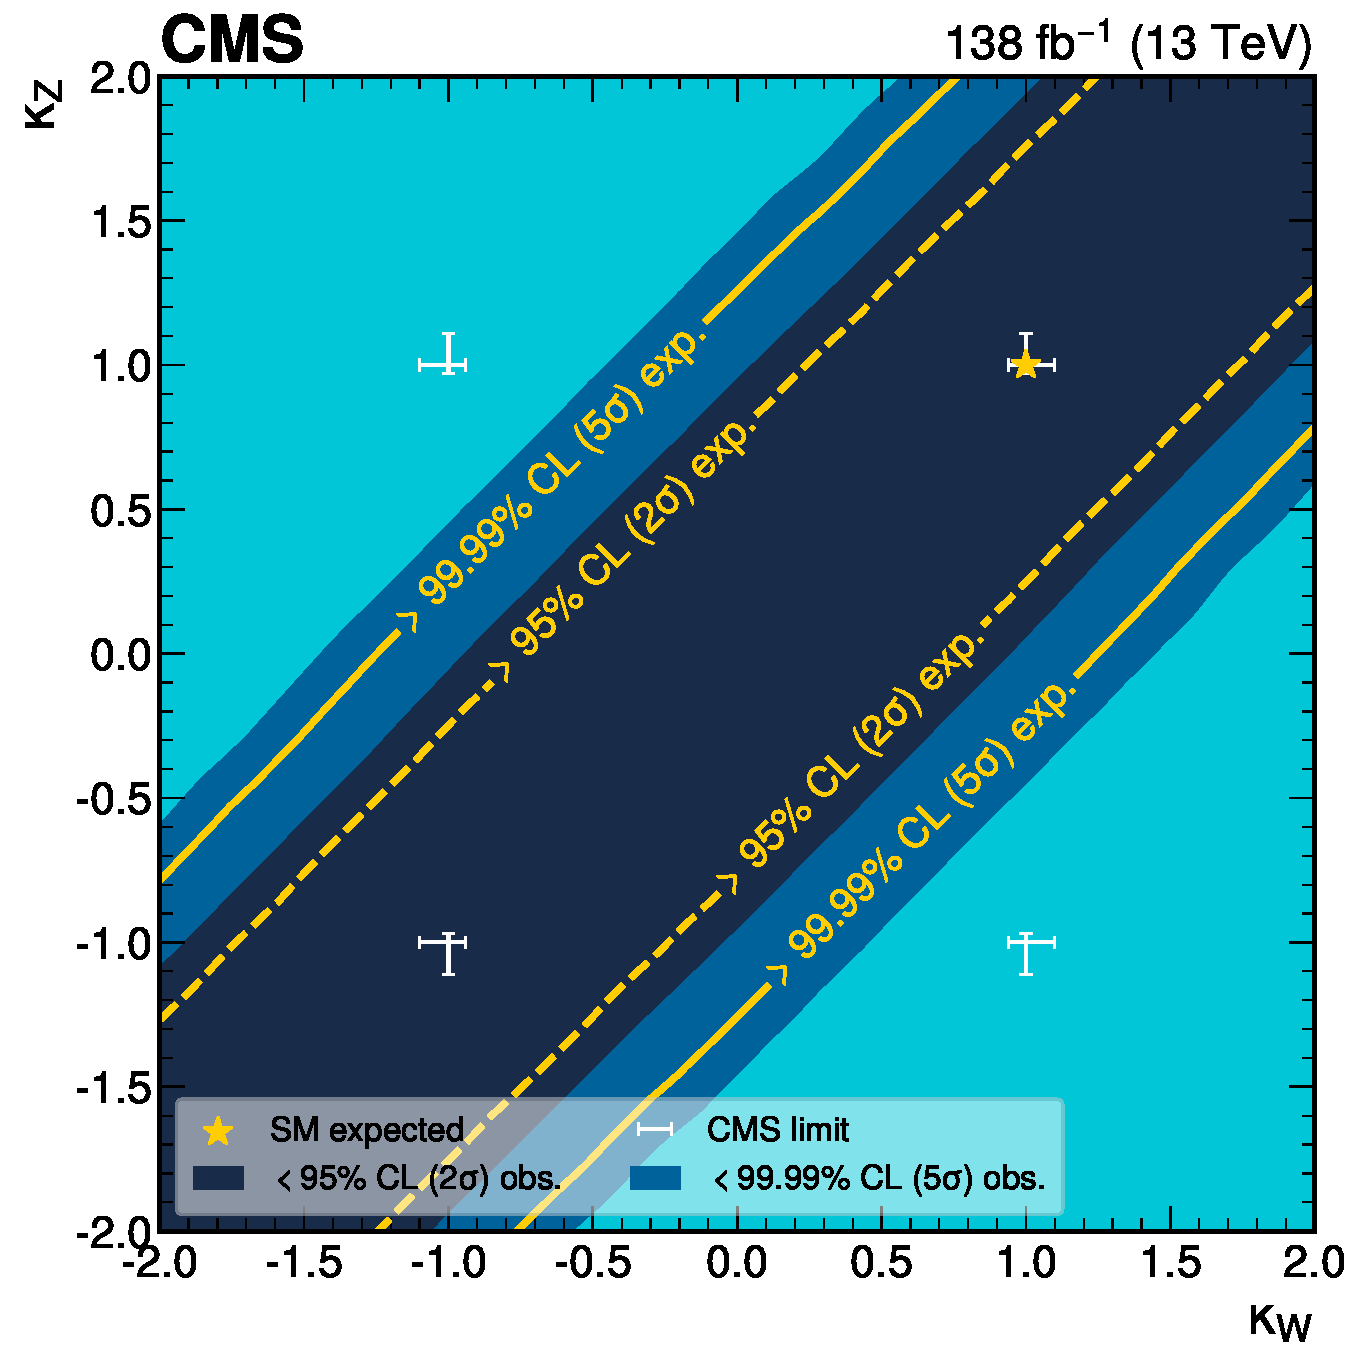
\includegraphics[width=0.5\textwidth]{fig/vbswh/exclusion_2D_contours_unblinded.pdf}
    \caption{
        Exclusion significance plotted as a function of \kW and \kZ.
        Opposite-sign scenarios ($\lambdaWZ < 0$) are excluded well beyond 5$\,\sigma$. 
    }
    \label{fig:vbswh_limit}
\end{figure}

\section{Measurement of \kVV through VBS VVH}
\subsection{Motivation}
\begin{figure}[htb]
    \centering
    \subfloat{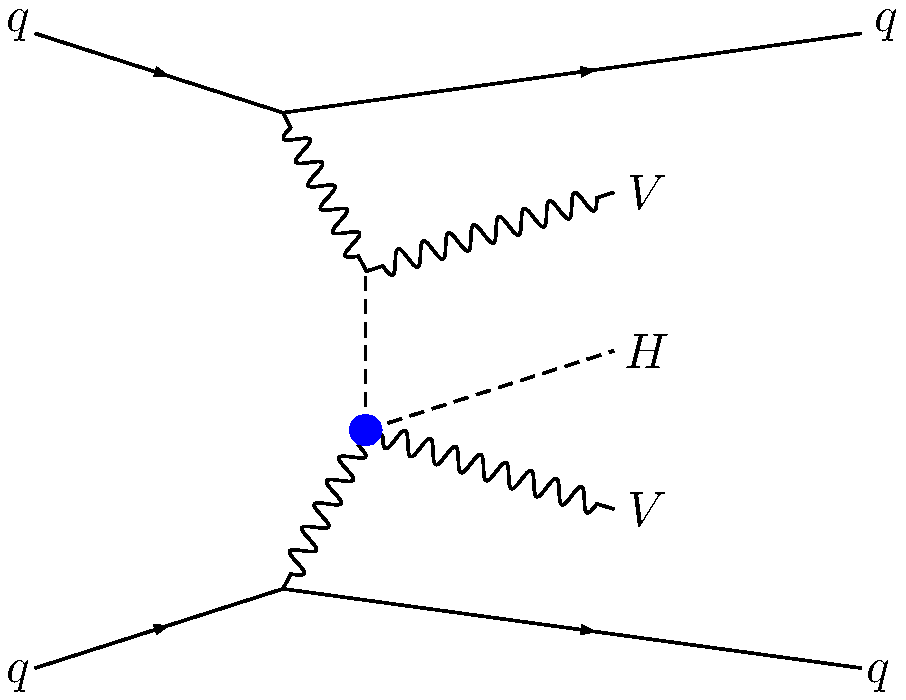
\includegraphics[width=0.3\textwidth]{fig/feynman/vbsvvh/vbsvvh_c2v.pdf}}\quad
    \subfloat{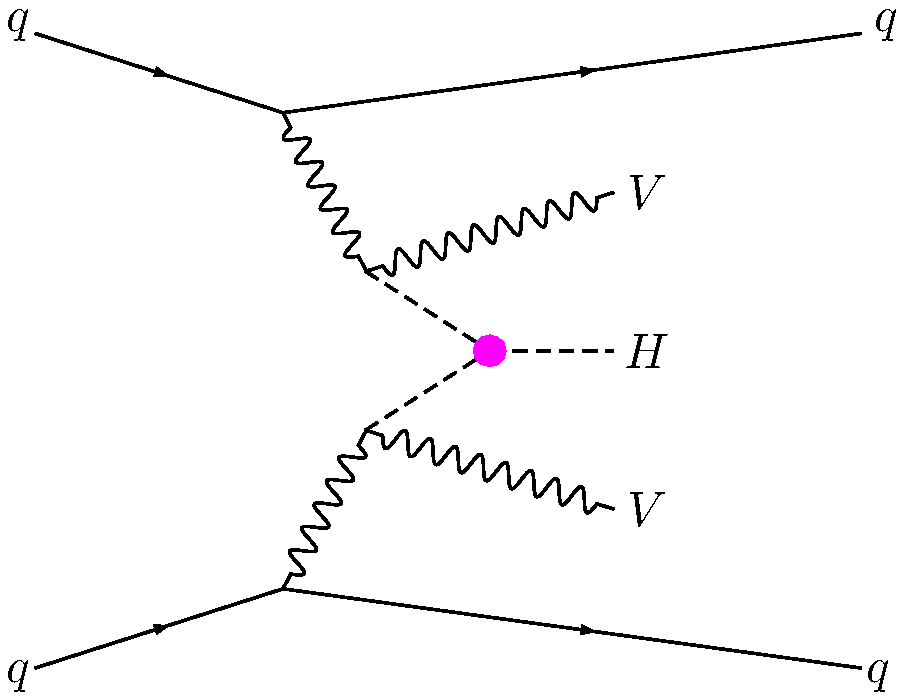
\includegraphics[width=0.3\textwidth]{fig/feynman/vbsvvh/vbsvvh_c3.pdf}}\quad
    \caption{
        Leading-order Feynman diagrams for VBS production of two vector bosons (V) and one Higgs boson. 
        The HHVV coupling \kVV is denoted by a blue circle (\textcolor{blue}{\ding{108}}), and the HHH coupling \kHHH is denoted by a magenta circle (\textcolor{magenta}{\ding{108}}). 
    }
    \label{fig:vbsvvh_feynman}
\end{figure}
\subsection{The signal}
\begin{figure}[htb]
    \centering
    \subfloat{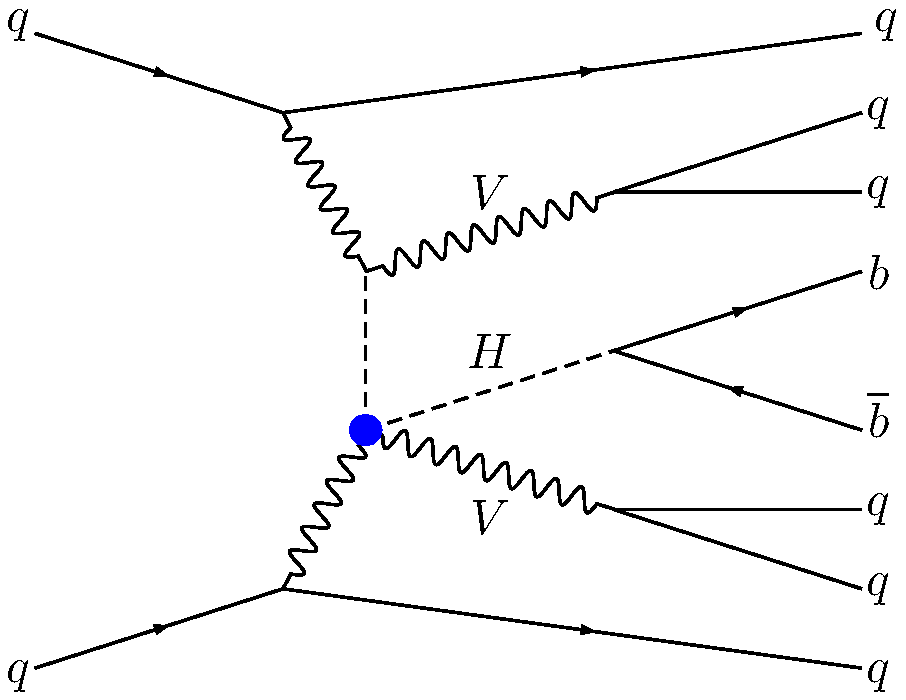
\includegraphics[width=0.3\textwidth]{fig/feynman/vbsvvh/vbsvvh_c2v_allhad.pdf}}\quad
    \subfloat{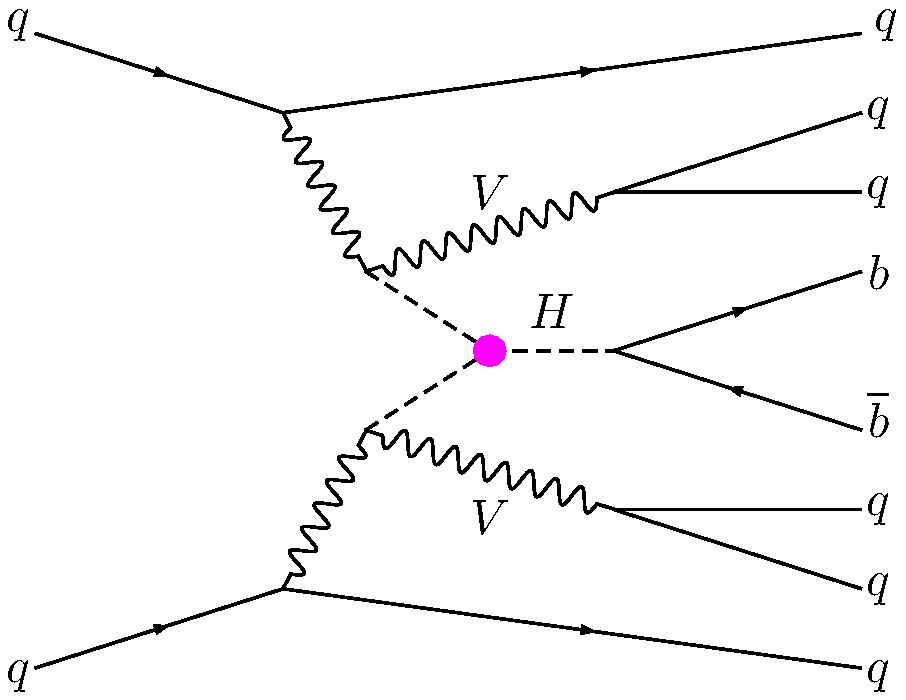
\includegraphics[width=0.3\textwidth]{fig/feynman/vbsvvh/vbsvvh_c3_allhad.pdf}}\quad
    \caption{
        Leading-order Feynman diagrams for VBS production of two vector bosons (V) and one Higgs boson, where the vector bosons decay hadronically and the Higgs boson decays specifically to b quarks. 
        The HHVV coupling \kVV is denoted by a blue circle (\textcolor{blue}{\ding{108}}), and the HHH coupling \kHHH is denoted by a magenta circle (\textcolor{magenta}{\ding{108}}). 
    }
    \label{fig:vbsvvh_feynman_allhad}
\end{figure}
\subsection{The backgrounds}
\subsection{Event selection}
\subsection{ABCDNet}
\subsection{Background estimation}
\subsection{Results}
